% chktex-file 3 chktex-file 9 chktex-file 17 chktex-file 18 chktex-file 36

\section{Modelos ARIMA y SARIMA}

Recuerde la definición de los operadores $\nabla^d = (I-B)^d$ y $\nabla_s^D = (I-B^s)^D$.

\subsection*{9.1 Definición Modelos ARIMA}

Para un número natural $d \geq 0$, se dice que $\{X_t\}$ es un proceso $\ARIMA(p,d,q)$ (Auto-regressive integrated moving average) si al definir $Y_t := \nabla^d X_t$ obtenemos un proceso $\ARMA(p,q)$
\[ \phi(B) Y_t = \phi(B)(1-B)^d X_t = \theta(B) Z_t,\quad Z_t \sim \WN(0,\sigma^2), \]
con $\phi$ y $\theta$ polinomios de grado $p$ y $q$ respectivamente.

\subsection*{9.6 Definición Modelos SARIMA}

Note que si hay un componente estacional en el proceso estocástico, donde cada ciclo o temporada dura $s$ unidades. Entonces aplicar el operador $\nabla_s$ debería remover en alguna medida el efecto de este componente como si discutió en el capítulo 1. Sin embargo, el patrón que sigue de un ciclo a otro podría ser aleatorio.

\begin{figure}[H]
    \centering
    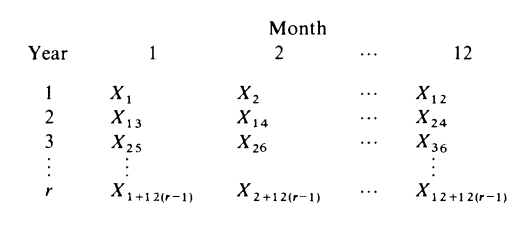
\includegraphics[width=0.55\textwidth]{../pictures/image5.png}
\end{figure}

Por ejemplo, la forma en la que se puede comportar una variable aleatoria de un año $y \in \Z$ hacia atrás podría representar otro proceso $\ARMA(P,Q)$ en donde si $X_{y}^{(m)} = X_{m+12y}$, entonces para cada mes $m = 1,\ldots 12$
\[ X_{y}^{(m)} - \Phi_1 X_{y-1}^{(m)} - \cdots - \Phi_{P} X_{y-P}^{(m)} = U_{y}^{(m)} + \Theta_1 U_{y-1}^{(m)} + \cdots + \Theta_1 U_{y-Q}^{(m)}, \]
para $U_{y}^{(m)} \sim \WN(0, \sigma_U^2)$. 

Si en particular, después de aplicar $\nabla^d \nabla_s^D$ para $d, D \in \N$ obtenemos un proceso $\ARMA(p,q)$ causal $Y_t := (I-B)^d (I-B^s)^D$, entonces podemos escribir
\[ \phi(B) \Phi(B^s) Y_t = \theta(B) \Theta(B^s) Z_t,\quad Z_t \sim \WN(0,\sigma^2). \]

Si el proceso cumple las condiciones mencionadas anteriormente, entonces decimos que es un proceso $\SARIMA(p,d,q)\times (P,D,Q)_s$.



\subsection*{9.2 Técnicas de Identificación}

Los desafíos de este capítulo son:
\begin{itemize}
    \item[(a)] Hallar una forma de transformar un proceso estocástico $X_t$ para obtener una serie de tiempo estacionaria y consecuentemente un proceso $\ARMA$.
    \begin{itemize}
        \item Aplicar (si es posible) alguna función $f$ que convierta una serie de tiempo en un proceso $\SARIMA$
        \item Hallar el periodo $s$ de componentes estacionales.
        \item Hallar $D$ que al diferenciar con $\nabla_s^D$ elimine tendencias en el componente estacional.
        \item Hallar $d$ que al diferenciar con $\nabla_d$ elimine tendencias globales. (9.1)
    \end{itemize}
    \item[(b)] Para una serie de tiempo a la cual se le quiere ajustar un proceso $\ARMA(p,q)$, la escogencia de $p,q$ son fundamentales para la precisión de futuras predicciones
    \begin{itemize}
        \item Escoger $p,q$ muy grandes puede llevar a sobreajustes, así que se requieren criterios de selección óptimos y eficientes de calcular. (9.3)
    \end{itemize}
    \item[(c)] Estimar un modelo ARMA (8.4 y 8.7) y arreglar este ajuste con residuales (9.4)
    \begin{itemize}
        \item Lo preferible es obtener para $Z_t \sim \WN(0,\hat{\sigma}^2)$ un ajuste $\phi(B) X_t = \theta(B) Z_t$. Queremos ver si este es el caso con los residuales
        \item Si obtenemos $\phi(B) X_t = \theta(B) Z_t$, y los residuales nos indican que $Z_t$ no es de ruido blanco, pero en cambio existe $\phi_Z$ y $\theta_Z$ tal que
        \[ \phi_Z(B) Z_t = \theta_Z(B) Z'_t,\quad Z_t' \sim \WN(0,\sigma'^{2}), \]
        entonces reajustamos el proceso para obtener los coeficientes correctos del modelos $\ARMA$ para $X_t$
        \[ \phi_Z(B) \phi(B) X_t = \phi_Z(B) \theta(B) Z_t = \theta_Z(B) \theta(B) Z_t'. \]
    \end{itemize}
\end{itemize}

\begin{figure}[H]
    \centering
    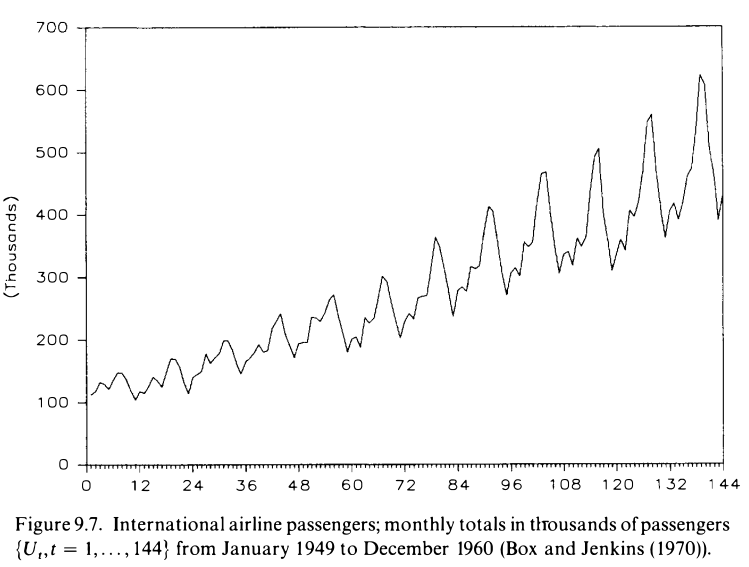
\includegraphics[width=0.45\textwidth]{../pictures/image1.png}
    \hfill
    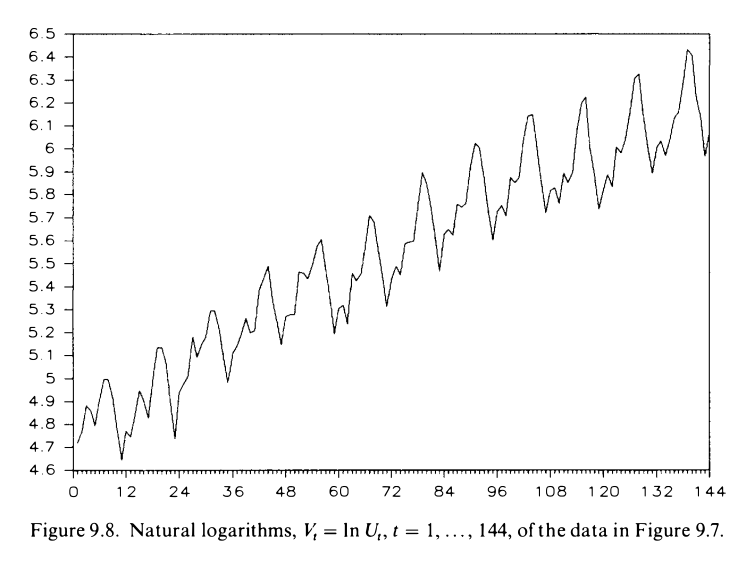
\includegraphics[width=0.45\textwidth]{../pictures/image2.png}
\end{figure}


\begin{figure}[H]
    \centering
    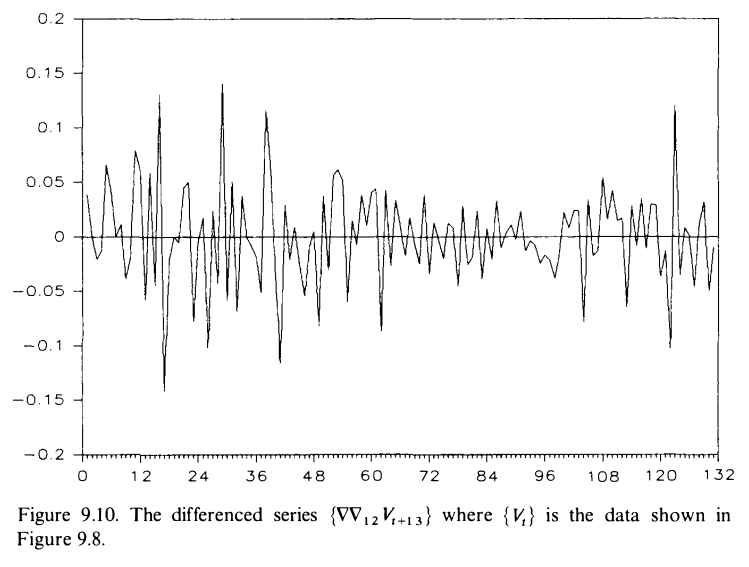
\includegraphics[width=0.45\textwidth]{../pictures/image3.png}
    \hfill
    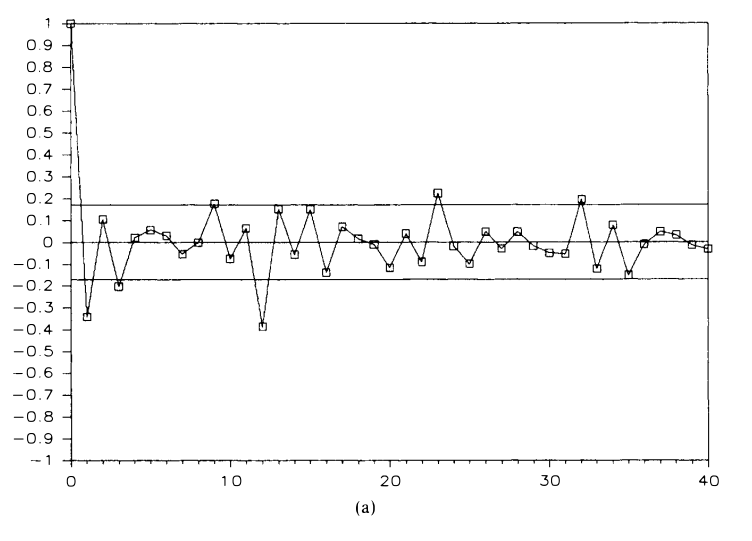
\includegraphics[width=0.45\textwidth]{../pictures/image4.png}
\end{figure}

La última gráfica corresponde a la función de autocorrelación de la serie $\nabla \nabla_{12} V_{t+13}$. 

Si se observa un crecimiento de la varianza a lo largo del tiempo de forma lineal, se puede remover este crecimiento aplicando un logaritmo al proceso.

A partir de la diferenciación con el operador $\nabla$ se puede eliminar tendencias lineales y con el operador $\nabla_s$ se puede eliminar estacionalidad ("seasonality") de periodo $s$ de un proceso estocástico $X_t$.

\subsection*{9.5 Predicciones de Modelos ARIMA}

Sea $X_t$ un proceso $\ARIMA(p,d,q)$, queremos predecir futuros valores de $X_t$. Sin embargo, las herramientas que hemos desarrollado solo sirven para procesos $\ARMA$, así que se requieren algunas modificaciones.

Si $(1-B)^d X_t =: Y_t$ en donde $Y_t$ es un modelos $\ARMA(p,q)$, entonces podemos reescribir la ecuación de la siguiente forma
\[ X_t = Y_t - \sum_{j = 1}^{d} \binom{d}{j} (-1)^j  X_{t-j}. \tag{9.5.1}\]
Si $X_{1-d},X_{2-d},\ldots,X_n$ es una realización de $X_t$, entonces los valores observados de $Y_t$ son $Y_1,\ldots, Y_n$. Defina
\[ S_n = \ol{\sp}\{X_{1-d},X_{2-d},\ldots,X_n\}, \]
y note que el mejor predictor lineal de $X_{n+h}$ basado en las $n+d$ observaciones de $X_t$ es $P_n X_{n+h} := P_{S_n} X_{n+h}$. Luego, definimos
\[ P_n Y_{n+h} := P_{\ol{\sp}\{Y_1,\ldots, Y_n\}} Y_{n+h} \]
\[ \wh{Y}_{n+1} := P_{\ol{\sp}\{Y_1,\ldots, Y_n\}} Y_{n+1} = P_n Y_{n+1} \]
y para continuar, debemos asumir que no hay correlación entre $X_{1-d},\ldots, X_0$ y $Y_t$ para $t > 0$, de esta forma
\[ \ol{\sp}\{X_{1-d},X_{2-d},\ldots,X_0\} \perp \ol{\sp}\{Y_{1},Y_{2},\ldots,Y_n\}, \]
y por ende, obtenemos con $(9.5.1)$ que
\[ S_n = \ol{\sp}\{X_{1-d},\ldots,X_0, Y_1, \ldots, Y_n\}.  \]
Por lo tanto,
\[ P_{S_n} Y_{n+h} = P_{S_0} Y_{n+h} + P_n Y_{n+h} = P_n Y_{n+h}. \tag{9.5.2}\]
Luego podemos recursivamente computar $P_{S_n}X_{n+h}$ con la siguiente fórmula

\[ P_{S_n} X_{n+h} = P_n Y_{n+h} - \sum_{j = 1}^{d} \binom{d}{j}(-1)^j P_{S_n} X_{n+h-j}.  \tag{9.5.3}\]

Para el MSE "Mean squared error" defina
\[ X_{n+1}^* = P_{S_n} X_{n+1}, \]
y note que
\[ X_{n+1} - X_{n+1}^* = Y_{n+1} - \wh{Y}_{n+1} \]
Luego, al aplicar innovaciones en $Y_t$ (ver 5.3.9) obtenemos para $n > m = \max(p,q)$ y $h \geq 1$ lo siguiente:
\[ \everymath{\displaystyle}
\arraycolsep=1.8pt\def\arraystretch{2.5}
\begin{array}{rcl}
    P_n Y_{n+h} & = & \sum_{i = 1}^{p}\phi_i P_n Y_{n+h-i} + \sum_{j = h}^1 \theta_{n+h-1,j} (Y_{n+h-j} - \wh{Y}_{n+h-j})\\
    & = & \sum_{i = 1}^{p}\phi_i P_n Y_{n+h-i} + \sum_{j = h}^1 \theta_{n+h-1,j} (X_{n+h-j} - X_{n+h-j}^*)
\end{array} \tag{9.5.4} \]
Por lo tanto, mezclando (9.5.2), (9.5.3) y (9.5.4) obtenemos
\[ P_{S_n} X_{n+h} = \sum_{j = 1}^{p+d} \psi_j^* P_{S_n} X_{n+h-j} + \sum_{j = h}^q \theta_{n+h-1,j} (X_{n+h-j} - X_{n+h-j}^*).\]

Luego, (Problema 9.9) se sigue que
\[ \sigma_n^2(h) = \E[(X_{n+h} - P_{S_n} X_{n+h})^2] = \sum_{j = 0}^{h-1} \left( \sum_{r = 0}^j \chi_r \theta_{n+h-r-1,j-r} \right)^2 v_{n+h-j-1}. \]

En donde $\theta_{n0} = 1$, $\chi(z) = \chi_0 + \chi_1 z + \cdots = ((1-z)^d \phi(z))^{-1}$ para $|z| < 1$, y
\[ v_{n+h-j-1} = \E[(X_{n+h-j - X_{n+h-j}^*})^2] = \E[(Y_{n+h-j} - \wh{Y}_{n+h-j})^2] \]
